\documentclass[11pt,a4paper]{article}

\usepackage[margin=2.4cm]{geometry}
\usepackage[T1]{fontenc}
\usepackage{lmodern}
\usepackage{microtype}
\usepackage{amsmath,amssymb,amsthm}
\usepackage{graphicx}
\usepackage{booktabs}
\usepackage{caption}
\usepackage{xcolor}
\usepackage[hidelinks]{hyperref}
\usepackage{url}
\usepackage{float}

\captionsetup{font=small,labelfont=bf,width=0.95\linewidth}
\setlength{\parskip}{0.4em}
\setlength{\parindent}{0pt}
\renewcommand{\arraystretch}{1.12}

\newtheorem{proposition}{Proposition}
\newtheorem{corollary}{Corollary}
\theoremstyle{definition}
\newtheorem{definition}{Definition}
\theoremstyle{remark}
\newtheorem{remark}{Remark}

\newcommand{\Prob}{\mathbb{P}}
\newcommand{\F}{\mathcal{F}}
\newcommand{\1}{\mathbf{1}}
\newcommand{\EXTEN}{7.1}
\newcommand{\EXTWENTYFIVE}{1.3}
\newcommand{\EXFIFTY}{0.2}
\newcommand{\UTenLo}{45}
\newcommand{\UTenHi}{59}
\newcommand{\UTwentyFiveLo}{45}
\newcommand{\UTwentyFiveHi}{56}
\newcommand{\TailDayLongPC}{6.8\%}
\newcommand{\TailDayLongPP}{14.3\%}
\newcommand{\TailDayLongPCTwentyFive}{26.3\%}
\newcommand{\TailDayLongPPTwentyFive}{51.5\%}
\newcommand{\TailDayShortPC}{7.0\%}
\newcommand{\TailDayShortPP}{17.0\%}
\newcommand{\MajorsDayU}{70}
\newcommand{\TailHourPPTen}{0.64\%}
\newcommand{\TailHourPPTwentyFive}{3.9\%}
\newcommand{\TailHourPPFifty}{31.6\%}
\newcommand{\TailHourPCTen}{0.30\%}
\newcommand{\TailHourPCTwentyFive}{1.9\%}
\newcommand{\TailHourPCFifty}{15.9\%}
\newcommand{\TailDayPPFifty}{81.0\%}
\newcommand{\TailDayPCFifty}{43.4\%}
\newcommand{\LargeDayPPTwentyFive}{40.5\%}
\newcommand{\LargeDayPCTwentyFive}{20.6\%}
\newcommand{\LevULo}{45}
\newcommand{\LevUHi}{54}
\newcommand{\KappaLo}{1.20}
\newcommand{\KappaHi}{1.63}
\newcommand{\LargeHourQC}{3.8\%}
\newcommand{\LargeHourQP}{5.4\%}
\newcommand{\RWExLo}{9}
\newcommand{\RWExHi}{47}
\newcommand{\LongKappaExLo}{21}
\newcommand{\LongKappaExHi}{44}
\newcommand{\ShortKappaExHi}{63}
\newcommand{\NewDayShortQC}{30.4\%}
\newcommand{\NewDayShortQP}{49.5\%}
\newcommand{\LevCloseLargeHour}{17}
\newcommand{\LevPathLargeHour}{14}
\newcommand{\LevCloseTailDayShort}{4.0}
\newcommand{\LevPathTailDayShort}{2.7}
\newcommand{\CohortMaxDK}{0.05}
\newcommand{\CohortMaxDU}{3}
\newcommand{\RobLargeMark}{51}
\newcommand{\RobLargeLast}{58}
\newcommand{\RobTailMark}{52}
\newcommand{\RobTailLast}{60}
\newcommand{\MMRBTC}{0.4\%}
\newcommand{\MMRMedian}{2.0\%}
\newcommand{\MMRMax}{17\%}
\newcommand{\FallbackN}{1}
\newcommand{\ListingsN}{312}
\newcommand{\DelistingsN}{91}
\newcommand{\ListingsPerMonth}{26.0}
\newcommand{\DelistingsPerMonth}{7.6}
\newcommand{\ListingsMin}{12}
\newcommand{\ListingsMax}{58}
\newcommand{\DelistingsMin}{1}
\newcommand{\DelistingsMax}{18}


\title{\textbf{Path-Dependent Liquidation Risk in Crypto Perpetual Futures}\\[0.3em]
\large On the Inadequacy of Close-to-Close Volatility under Continuous Margin Monitoring:\\
Evidence from 753 Binance USDT-Margined Perpetuals, November 2025 -- October 2026}
\author{Ricardo P\'erez Twerdy\thanks{Contact: \href{mailto:rtwerdy@gmail.com}{rtwerdy@gmail.com}.
This paper is independent research. It is not affiliated with, sponsored by, or related in any way
to the author's work at Coinbase, and it does not represent the views of Coinbase. Nothing in it is
investment advice.}}
\date{November 2026}

\begin{document}
\maketitle

\begin{abstract}
\noindent Risk measures for leveraged positions are routinely estimated from close-to-close
returns, while liquidation engines in crypto perpetual futures monitor the mark price continuously
and liquidate at the first touch of the liquidation boundary. We formalise the gap as the
difference between a first-passage event and a terminal event, and derive its Brownian benchmarks:
half of all boundary crossings are invisible at the horizon end, and the 99th-percentile path loss
exceeds the terminal loss by a factor of $1.107$. We then measure both quantities on 12 months of
1-minute mark-price data for every USDT-margined perpetual listed on Binance, using a
point-in-time universe that includes delisted contracts. At 10x leverage, 45--59\% of liquidations
occur in holding windows that end inside the liquidation boundary, in every liquidity tier outside
BTC and ETH. The 99th-percentile adverse excursion is 1.20 to 1.63 times the 99th-percentile
close-to-close loss, well above the Brownian benchmark, and is largest for short positions in newly
listed contracts. The results hold on a balanced cohort of surviving contracts. With leverage of up
to 150x available on major venues and a median contract offering 20--25x, the gap between the two
measures is economically first-order.
\end{abstract}

\section{Introduction}

A volatility estimate built from closing prices answers the question \emph{how far apart are two
closing prices?} A leveraged position faces a different question: \emph{how far does the price
travel against the position before it can be closed?} In markets that close, settle margin on
closing prices and are monitored at discrete times, the two questions are close. Crypto perpetual
futures differ in three ways. The market never closes, so a daily ``close'' is an arbitrary
timestamp. Liquidation engines monitor the mark price continuously and act within seconds. And a
position liquidated at 03:00 is closed, whatever the price does by midnight.

\paragraph{Leverage.} The consequence is amplified by the leverage on offer
(Table~\ref{tab:venues}). Binance and Bybit allow up to 150x on their BTC and ETH perpetuals, OKX
up to 100x, Deribit up to 50x on its linear USDC perpetuals, and Hyperliquid up to 40x. Leverage
on smaller contracts is lower but far from modest: the median contract allows 25x on Binance and
Bybit and 20x on OKX, and between 17\% and 37\% of contracts on these three venues allow 50x or
more. At $L$-fold leverage the liquidation boundary lies roughly $1/L$ from entry: about 10\% at
10x, 4\% at 25x and 2\% at 50x. Liquid crypto assets make such moves within hours, often within
minutes. Binance, Bybit, OKX and Hyperliquid all document that liquidation is triggered by a mark
price rather than by the last traded price~\cite{binance-liq,bybit-mark,okx-liq,hl-liq}; our
analysis therefore uses Binance's mark price throughout.

\begin{table}[t]
\centering
\caption{Maximum leverage on linear (USDT- or USDC-margined) perpetuals, retrieved from each
venue's public market-data interface on 22 November 2026. \emph{BTC}: the venue's linear BTC
perpetual. \emph{Median}, $\geq$\,50x, $\leq$\,10x: across all listed contracts. Binance values are
for the first (smallest-notional) risk bracket. Sources:
\cite{binance-brackets,bybit-api,okx-api,deribit-api,hl-api}.}
\label{tab:venues}
\small
\begin{tabular}{@{}lrrrrrr@{}}
\toprule
Venue & Contracts & BTC & Highest & Median & $\geq$ 50x & $\leq$ 10x \\
\midrule
Binance & 930 & 150x & 150x & 25x & 37\% & 22\% \\
Bybit & 831 & 150x & 150x & 25x & 23\% & 5\% \\
OKX & 531 & 100x & 100x & 20x & 17\% & 28\% \\
Deribit & 152 & 50x & 50x & 10x & 14\% & 55\% \\
Hyperliquid & 179 & 40x & 40x & 5x & 0\% & 98\% \\
\bottomrule
\end{tabular}

\end{table}

\paragraph{An example.} Figure~\ref{fig:example} shows one 24-hour window on BTCUSDT, the most
liquid perpetual in the market. A long position opened at 17:00 UTC on 5 February 2026 ended the
window \textbf{2.4\% above entry}. A close-to-close risk model records a profitable, unremarkable
day. Along the way the mark price fell 12.1\% below entry: a 50x long was liquidated after
\EXFIFTY{} hours (twelve minutes), a 25x long after \EXTWENTYFIVE{} hours and a 10x long after \EXTEN{} hours.

\begin{figure}[t]
\centering
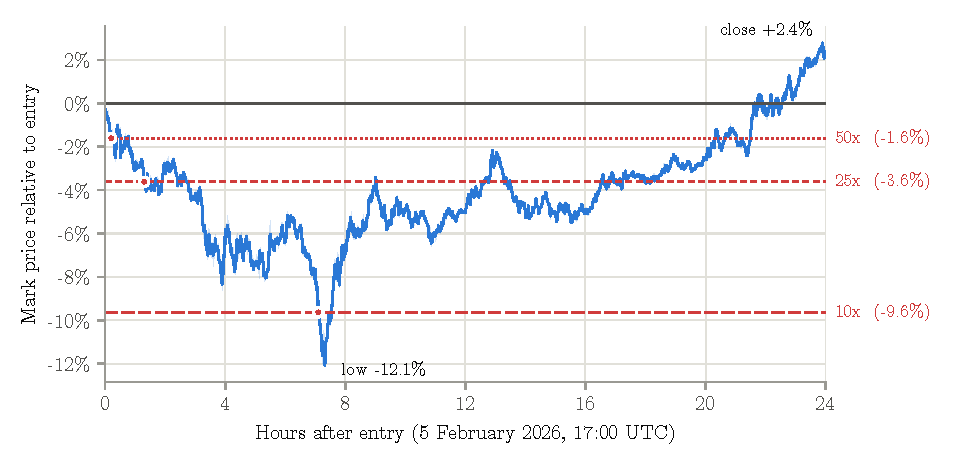
\includegraphics[width=\linewidth]{figures/fig1_example.pdf}
\caption{BTCUSDT mark price relative to entry, 24 hours from 5 February 2026 17:00 UTC. The
shaded band is each minute's high--low range. Dashed lines: liquidation boundaries of isolated
longs at 10x, 25x and 50x with a 0.4\% maintenance-margin rate (Section~\ref{sec:liq}); dots mark
the first touch of each. A close-to-close model sees $+2.4\%$.}
\label{fig:example}
\end{figure}

\paragraph{Contribution.} We (i) formalise liquidation as a first-passage event and the
close-to-close view as a terminal event, and derive their Brownian benchmarks
(Section~\ref{sec:framework}); (ii) build a point-in-time, survivorship-free universe of 753
Binance perpetuals over 12 months (Section~\ref{sec:data}); and (iii) measure, across liquidity
tiers, horizons, sides and leverage levels, how often liquidations are unseen at the close and how
much heavier the tail of the path is than the tail of the close (Sections~\ref{sec:results}
and~\ref{sec:robust}).

\section{Stochastic framework}
\label{sec:framework}

\subsection{Setting}

Let $(\Omega,\F,\mathbb{F},\Prob)$ be a filtered probability space, with filtration
$\mathbb{F}=(\F_t)_{t\ge 0}$ satisfying the usual conditions. The mark price $(M_t)_{t\ge0}$ of a
perpetual contract is a strictly positive, $\mathbb{F}$-adapted process with c\`adl\`ag paths. A
position opened at time $t_0$ and held for a horizon $h>0$ has log-return process
\begin{equation}
X_t = \log\frac{M_{t_0+t}}{M_{t_0}}, \qquad 0\le t\le h,
\end{equation}
with running minimum and maximum $\underline{X}_h=\inf_{0\le t\le h}X_t$ and
$\overline{X}_h=\sup_{0\le t\le h}X_t$.

A long position is liquidated when the mark price falls by a fraction $d_\ell\in(0,1)$ from entry,
and a short when it rises by $d_s>0$ (Section~\ref{sec:liq} derives $d_\ell$ and $d_s$). In log
terms the boundaries are $b_\ell=-\log(1-d_\ell)$ and $b_s=\log(1+d_s)$.

\begin{definition}[Liquidation time]
The liquidation time of a long position is the first-passage time
\begin{equation}
\tau_\ell=\inf\{t\in[0,h]: X_t\le -b_\ell\}, \qquad \inf\emptyset=+\infty,
\end{equation}
and analogously $\tau_s=\inf\{t\in[0,h]:X_t\ge b_s\}$ for a short. Since $X$ is c\`adl\`ag and
adapted and $\mathbb{F}$ satisfies the usual conditions, $\tau_\ell$ and $\tau_s$ are stopping times
(the d\'ebut theorem).
\end{definition}

\begin{definition}[Path and close breaches]
For a long position, the \emph{path breach} is the event $A_P=\{\tau_\ell\le h\}=\{\underline{X}_h\le
-b_\ell\}$ and the \emph{close breach} is the event $A_C=\{X_h\le -b_\ell\}$, with probabilities
$p_P=\Prob(A_P)$ and $p_C=\Prob(A_C)$. Since $X_h\ge\underline{X}_h$, $A_C\subseteq A_P$. The
\emph{unseen share} is the fraction of liquidations that a close-to-close observer does not record:
\begin{equation}
U=\Prob\big(A_C^{c}\,\big|\,A_P\big)=1-\frac{p_C}{p_P}.
\end{equation}
For a level $\alpha\in(\tfrac12,1)$, the \emph{path-to-close quantile multiple} is
\begin{equation}
\kappa_\alpha=\frac{Q_\alpha\big(-\underline{X}_h\big)}{Q_\alpha\big(-X_h\big)},
\end{equation}
where $Q_\alpha$ denotes the $\alpha$-quantile. Short positions use $\overline{X}_h$, $X_h$ and
$b_s$ symmetrically.
\end{definition}

$U$ measures how often a close-to-close view misses a liquidation; $\kappa_\alpha$ measures by how
much it understates the tail of the adverse move. Neither requires a model of $M$, and both have
exact benchmarks under Brownian motion.

\subsection{The Brownian benchmark}

Suppose $X_t=\sigma W_t$, with $W$ a standard $\mathbb{F}$-Brownian motion and $\sigma>0$.

\begin{proposition}[Reflection principle]
\label{prop:reflection}
For every $b>0$,
\begin{equation}
\Prob\big(\underline{X}_h\le -b\big)=2\,\Prob\big(X_h\le -b\big)=2\,\Phi\!\left(-\frac{b}{\sigma\sqrt h}\right),
\end{equation}
where $\Phi$ is the standard normal distribution function.
\end{proposition}

\begin{proof}[Sketch]
Let $\tau=\inf\{t:W_t=-b/\sigma\}$. On $\{\tau\le h\}$, the strong Markov property and the
symmetry of Brownian increments give $\Prob(W_h\le -b/\sigma\mid\F_\tau)=\tfrac12$. Since
$\{X_h\le -b\}\subseteq\{\tau\le h\}$, it follows that $\Prob(X_h\le-b)=\tfrac12\Prob(\tau\le h)$.
\end{proof}

\begin{corollary}
\label{cor:half}
Under Brownian motion, $U=\tfrac12$ for every boundary $b$, volatility $\sigma$ and horizon $h$:
half of all liquidations are invisible at the close, whatever the leverage.
\end{corollary}

\begin{proposition}[Quantile multiple]
\label{prop:kappa}
Under Brownian motion, $\kappa_\alpha=z_{(1+\alpha)/2}/z_\alpha$, where $z_p=\Phi^{-1}(p)$. In
particular, $\kappa_{0.99}=2.5758/2.3263=1.107$.
\end{proposition}

\begin{proof}
By Proposition~\ref{prop:reflection}, $\Prob(-\underline{X}_h>x)=2\Phi(-x/(\sigma\sqrt h))$ for
$x>0$. Setting this equal to $1-\alpha$ gives $Q_\alpha(-\underline{X}_h)=\sigma\sqrt h\,
z_{(1+\alpha)/2}$, while $Q_\alpha(-X_h)=\sigma\sqrt h\,z_\alpha$.
\end{proof}

\begin{remark}[Drift]
With drift, $X_t=\mu t+\sigma W_t$, the first-passage probability becomes
$\Phi\big(\tfrac{-b-\mu h}{\sigma\sqrt h}\big)+e^{-2\mu b/\sigma^2}\Phi\big(\tfrac{-b+\mu h}{\sigma\sqrt h}\big)$.
Over horizons of hours to a day, $\mu h$ is negligible relative to $\sigma\sqrt h$, and the
benchmarks above are unchanged to the precision reported here.
\end{remark}

\begin{remark}[Discrete monitoring]
If the path were observed only at times $k\Delta$, the observed minimum would exceed
$\underline{X}_h$ and touches between observations would be missed. Broadie, Glasserman and
Kou~\cite{bgk} show that discrete monitoring is equivalent, to first order, to shifting the
boundary outward by $\beta\sigma\sqrt\Delta$, with $\beta=-\zeta(\tfrac12)/\sqrt{2\pi}\approx0.5826$,
which lowers $U$ below $\tfrac12$. Our data record the highest and lowest mark price within each
minute, so the path is observed at the frequency at which the venue updates its mark price (a few
seconds). The effective $\Delta$ is small and the Brownian benchmark is close to $\tfrac12$.
\end{remark}

\subsection{Departures from the benchmark}

Real mark-price paths are not Brownian. Heavy-tailed returns, jumps, and transient dislocations
that revert (``wicks'', often caused by forced liquidations themselves) make the running extremum
heavier relative to the terminal value. They raise $\kappa_\alpha$ above $1.107$ and, when the
dislocation reverts within the horizon, raise $U$ above $\tfrac12$. Persistent trends act in the
opposite direction on $U$. The two statistics are therefore model-free diagnostics: $U$ measures
\emph{how often} the close misses the liquidation, and $\kappa_\alpha$ measures \emph{how far} the
close understates the adverse tail, each against an exact benchmark. Range-based volatility
estimators~\cite{parkinson,garmanklass,rogerssatchell} rest on the same observation: the extremes of
a path carry information that the close discards.

\section{Data and a point-in-time universe}
\label{sec:data}

\paragraph{Prices.} We use Binance USDT-margined perpetual futures from the public archive at
\url{https://data.binance.vision}: 1-minute mark-price candles, the price on which Binance
triggers liquidation~\cite{binance-liq}, and, for robustness, 1-minute last-traded-price candles.
The archive retains files for delisted contracts, so the sample is free of survivorship bias at the
source.

\paragraph{A universe that changes.} The set of tradable perpetuals in October 2026 differs from
the set in November 2025: 314 contracts were listed during the period and 89 stopped trading.
Fixing today's list and looking back would keep only the survivors. Instead, each date $t$ has its
own universe, built only from information available before $t$:
\begin{enumerate}\itemsep0pt
\item a contract enters on its listing day;
\item contracts younger than 30 days form the \emph{New} tier;
\item BTCUSDT and ETHUSDT form the \emph{Majors} tier;
\item the remaining contracts are ranked by trailing 30-day median daily turnover, using days
before $t$ only. The top 30 form the \emph{Large} tier; the rest form the \emph{Tail} tier if their
median turnover is at least \$5 million, and are otherwise excluded;
\item a contract leaves the universe at its last trade. The archive continues to publish flat,
zero-volume candles after a delisting; retaining them would add riskless windows.
\end{enumerate}
The tier \emph{definitions} are fixed while their \emph{membership} changes, as in an index
reconstitution. Ranking on the median rather than the mean prevents a single day of inflated
turnover from promoting a contract. Figure~\ref{fig:universe} and Table~\ref{tab:data} summarise the
universe.

\begin{figure}[t]
\centering
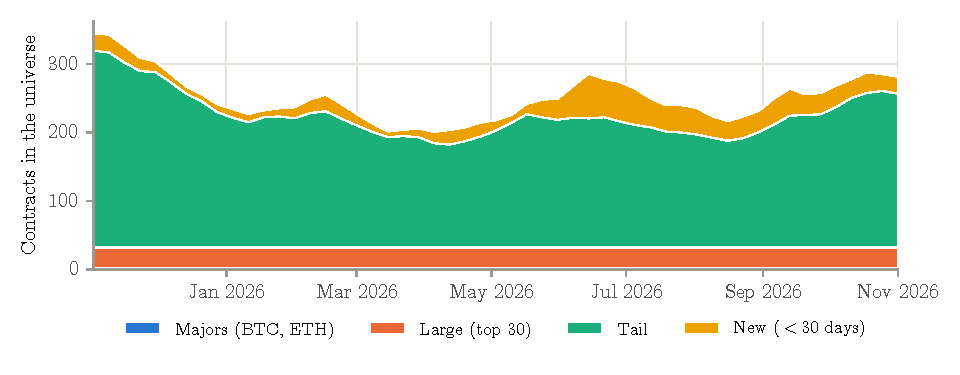
\includegraphics[width=\linewidth]{figures/fig5_universe.pdf}
\caption{Contracts in each tier, weekly mean of daily counts. The Majors tier (two contracts) is a
hairline at the bottom. New listings peaked in June and July 2026.}
\label{fig:universe}
\end{figure}

\begin{table}[t]
\centering
\caption{Data and universe, 1 November 2025 to 31 October 2026.}
\label{tab:data}
\small
\begin{tabular}{@{}lr@{}}
\toprule
Item & Value \\
\midrule
USDT-margined perpetuals in the archive (delisted included) & 924 \\
\quad with a listing date & 923 \\
\quad with 1-minute mark-price data in the study period & 900 \\
\quad in the point-in-time universe on at least one day & 753 \\
\quad of which delisted during the study & 42 \\
Balanced cohort (live for the whole study) & 424 \\
Mean contracts per day: majors / large / tail / new & 2 / 30 / 192 / 26 \\
Holding windows (1 h / 4 h / 8 h / 24 h), millions & 2.15 / 2.15 / 2.15 / 2.14 \\
\bottomrule
\end{tabular}

\end{table}

\section{Measurement}
\label{sec:measure}

\subsection{Holding windows}

Every hour, for every contract in the universe, we open a hypothetical long and a hypothetical
short at the mark price and hold each for $h\in\{1,4,8,24\}$ hours. For each window we record the
terminal log-return $X_h$ and the running extremes $\underline{X}_h$ and $\overline{X}_h$ from the
minute highs and lows. A window with any missing minute is discarded, never filled: a gap is
precisely where an unobserved extreme could lie.

\subsection{Liquidation boundary}
\label{sec:liq}

Consider isolated margin, a position of entry notional $N$ and leverage $L$, so that the initial
margin is $N/L$. A perpetual is delta-one, so profit and loss is linear in the relative price move
$x=M_{t_0+t}/M_{t_0}-1$: $+Nx$ for a long and $-Nx$ for a short.\footnote{We refer throughout to
linear (USDT- or USDC-margined) perpetuals, whose profit and loss is linear in the price. Inverse,
coin-margined perpetuals, such as Binance's COIN-M contracts or Deribit's BTC-PERPETUAL, settle
profit and loss in the base asset, $N(1-M_{t_0}/M_{t_0+t})$ for a long, which is not linear in the
price; their liquidation boundary differs and is not studied here.}
Liquidation occurs when equity falls to the maintenance margin, a fraction $m$ of the notional at the
current mark price:
\begin{align}
\text{long:}\quad & \tfrac{1}{L} + x = m(1+x) &&\Longrightarrow\quad d_\ell = \frac{1/L - m}{1-m},\\
\text{short:}\quad & \tfrac{1}{L} - x = m(1+x) &&\Longrightarrow\quad d_s = \frac{1/L - m}{1+m}.
\end{align}
A long survives slightly further than a short because its maintenance requirement falls as it
loses. A position is admissible only if $1/L>m$. We use one maintenance-margin rate per tier: 0.4\%
for Majors, 0.5\% for Large, and 1\% for Tail and New. The first two match Binance's current
first-bracket rates for BTCUSDT, ETHUSDT and SOLUSDT. The median first-bracket rate across all
Binance USDT perpetuals is 2\%~\cite{binance-brackets}, so our Tail and New boundaries lie further
from entry than the venue's, and the breach probabilities reported below are conservative.
Table~\ref{tab:liq} lists the boundaries. Fees, funding and liquidation penalties are ignored.

\subsection{Estimators and inference}

Let $\mathcal{D}$ be the set of days, $\mathcal{S}_t$ the contracts in a tier on day $t$, and
$W_{i,t}$ the windows of contract $i$ that start on day $t$. The close-breach probability is
estimated by
\begin{equation}
\hat p_C=\frac{1}{|\mathcal D|}\sum_{t\in\mathcal D}\frac{1}{|\mathcal S_t|}\sum_{i\in\mathcal S_t}
\frac{1}{|W_{i,t}|}\sum_{w\in W_{i,t}}\1\big\{X_h^{(w)}\le -b\big\},
\end{equation}
and $\hat p_P$ analogously, so that each contract counts once within a day and each day counts once
in the year; $\hat U=1-\hat p_C/\hat p_P$. Quantiles use the same weights. Windows are not
independent: hourly windows overlap, and market-wide moves affect all contracts at once. Confidence
intervals therefore come from a moving-block bootstrap that resamples whole days in blocks of seven,
preserving both the serial and the cross-sectional dependence. The effective sample size is the
number of days, 364, rather than the 8.6 million windows. The full measurement chain was validated
on simulated Brownian paths, where it reproduces the discretely monitored benchmark of Broadie,
Glasserman and Kou to within a few percent.

\section{Results}
\label{sec:results}

\subsection{About half of all liquidations are unseen at the close}

Table~\ref{tab:breach} reports, at 10x leverage, the close and path breach probabilities and the
unseen share. Outside the Majors tier, between \textbf{45\% and 59\%} of liquidations are unseen at
the close, in every tier, at every horizon and on both sides. The difference is large in absolute
terms: a 10x long in the Tail tier held for 24 hours ends beyond its liquidation boundary in 5.0\%
of windows, but is liquidated in 10.6\%; for a short, the figures are 5.5\% and 13.4\%.

\begin{table}[t]
\centering
\caption{Breach probabilities at 10x leverage, mark price. $p_C$: close breach; $p_P$: path breach
(liquidation); $U=1-p_C/p_P$: unseen share, with a 95\% block-bootstrap interval. ``--'': no close
breach in the sample.}
\label{tab:breach}
\footnotesize
\setlength{\tabcolsep}{4.2pt}
\begin{tabular}{@{}llrrlrrl@{}}
\toprule
 & & \multicolumn{3}{c}{Long, 10x} & \multicolumn{3}{c}{Short, 10x} \\
\cmidrule(lr){3-5}\cmidrule(lr){6-8}
Tier & $h$ & $p_C$ & $p_P$ & $U$ [95\% CI] & $p_C$ & $p_P$ & $U$ [95\% CI] \\
\midrule
Majors & 1 h & 0.00\% & 0.00\% & -- & 0.00\% & 0.00\% & -- \\
 & 8 h & 0.02\% & 0.14\% & 88\% \scriptsize[76\%, 100\%] & 0.02\% & 0.08\% & 79\% \scriptsize[77\%, 100\%] \\
 & 24 h & 0.33\% & 1.08\% & 70\% \scriptsize[57\%, 78\%] & 0.38\% & 0.86\% & 56\% \scriptsize[40\%, 77\%] \\
\addlinespace[2pt]
Large & 1 h & 0.13\% & 0.28\% & 51\% \scriptsize[46\%, 56\%] & 0.14\% & 0.32\% & 55\% \scriptsize[51\%, 58\%] \\
 & 8 h & 1.30\% & 2.88\% & 55\% \scriptsize[51\%, 58\%] & 1.53\% & 3.37\% & 55\% \scriptsize[53\%, 57\%] \\
 & 24 h & 4.37\% & 8.96\% & 51\% \scriptsize[49\%, 54\%] & 4.31\% & 9.54\% & 55\% \scriptsize[52\%, 57\%] \\
\addlinespace[2pt]
Tail & 1 h & 0.13\% & 0.29\% & 55\% \scriptsize[51\%, 59\%] & 0.18\% & 0.37\% & 53\% \scriptsize[51\%, 54\%] \\
 & 8 h & 1.43\% & 3.15\% & 55\% \scriptsize[52\%, 57\%] & 1.99\% & 4.61\% & 57\% \scriptsize[56\%, 58\%] \\
 & 24 h & 5.00\% & 10.59\% & 53\% \scriptsize[51\%, 54\%] & 5.50\% & 13.39\% & 59\% \scriptsize[57\%, 61\%] \\
\addlinespace[2pt]
New & 1 h & 0.31\% & 0.65\% & 52\% \scriptsize[46\%, 58\%] & 0.42\% & 0.90\% & 53\% \scriptsize[50\%, 56\%] \\
 & 8 h & 3.35\% & 6.60\% & 49\% \scriptsize[48\%, 51\%] & 3.14\% & 7.71\% & 59\% \scriptsize[57\%, 61\%] \\
 & 24 h & 9.29\% & 16.93\% & 45\% \scriptsize[43\%, 48\%] & 7.19\% & 17.55\% & 59\% \scriptsize[57\%, 61\%] \\
\bottomrule
\end{tabular}

\end{table}

Figure~\ref{fig:hidden} shows $U$ across leverage levels. It lies close to the Brownian value of
$\tfrac12$ almost everywhere, and a few points above it in most cells. The blind spot is therefore
\emph{structural}: a measure that looks only at the close misses about half of all liquidations
even under idealised dynamics (Corollary~\ref{cor:half}), and crypto price paths do not improve on
that. The Majors tier stands out, at 70\% for a 24-hour 10x long and 88\% at 8 hours, but on few
events and with wide intervals: BTC and ETH rarely move 10\% within a day.

\begin{figure}[t]
\centering
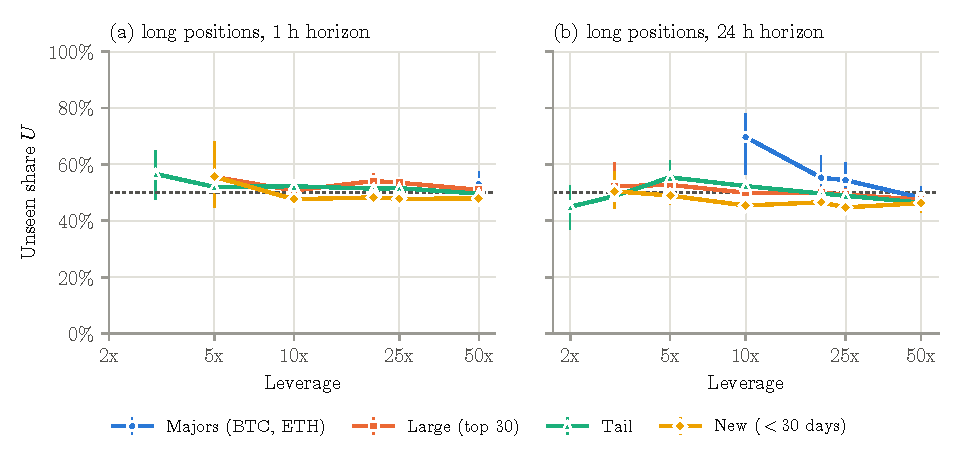
\includegraphics[width=\linewidth]{figures/fig2_hidden_share.pdf}
\caption{Unseen share $U$ for long positions, mark price, with 95\% block-bootstrap intervals.
Points whose interval is wider than 25 percentage points (too few close breaches) are omitted, which
removes most low-leverage Majors points. Dotted line: Brownian benchmark, $U=\tfrac12$.}
\label{fig:hidden}
\end{figure}

\subsection{At 10x, 25x and 50x}

Table~\ref{tab:leverage} sets the three leverage levels side by side for long positions. As leverage
rises, both breach probabilities rise steeply while $U$ stays near one half, so the \emph{number} of
liquidations a close-to-close view misses grows with leverage. For a long held one hour in the Tail tier, the liquidation probability is 0.29\% at 10x, 3.63\% at 25x and 26.2\% at 50x, against close-breach probabilities of 0.13\%, 1.77\% and 13.0\%. Held for 24 hours, a 50x long in the Tail tier is liquidated in 80.4\% of windows, while only 42.9\% end beyond the boundary; at 25x in the Large tier the figures are 39.1\% and 20.0\%. Outside the Majors tier the unseen share stays between 45\% and 55\% in every cell of the table. In the example of Figure~\ref{fig:example}, the 50x position was closed within twelve minutes of entry.

\begin{table}[t]
\centering
\caption{Long positions at 10x, 25x and 50x, mark price. $d_{\text{long}}$: adverse move to
liquidation. $p_C$, $p_P$: close and path breach probabilities; $U$: unseen share.}
\label{tab:leverage}
\footnotesize
\begin{tabular}{@{}llrrrrrrr@{}}
\toprule
 & & & \multicolumn{3}{c}{1 h} & \multicolumn{3}{c}{24 h} \\
\cmidrule(lr){4-6}\cmidrule(lr){7-9}
Tier & $L$ & $d_{\text{long}}$ & $p_C$ & $p_P$ & $U$ & $p_C$ & $p_P$ & $U$ \\
\midrule
Majors & 10x & 9.64\% & 0.00\% & 0.00\% & -- & 0.33\% & 1.08\% & 70\% \\
 & 25x & 3.61\% & 0.07\% & 0.22\% & 68\% & 7.39\% & 16.20\% & 54\% \\
 & 50x & 1.61\% & 1.17\% & 2.50\% & 53\% & 23.33\% & 44.99\% & 48\% \\
\addlinespace[2pt]
Large & 10x & 9.55\% & 0.13\% & 0.28\% & 51\% & 4.37\% & 8.96\% & 51\% \\
 & 25x & 3.52\% & 1.20\% & 2.56\% & 53\% & 19.98\% & 39.06\% & 49\% \\
 & 50x & 1.51\% & 6.13\% & 12.62\% & 51\% & 34.96\% & 66.04\% & 47\% \\
\addlinespace[2pt]
Tail & 10x & 9.09\% & 0.13\% & 0.29\% & 55\% & 5.00\% & 10.59\% & 53\% \\
 & 25x & 3.03\% & 1.77\% & 3.63\% & 51\% & 25.59\% & 50.36\% & 49\% \\
 & 50x & 1.01\% & 13.04\% & 26.17\% & 50\% & 42.87\% & 80.35\% & 47\% \\
\addlinespace[2pt]
New & 10x & 9.09\% & 0.31\% & 0.65\% & 52\% & 9.29\% & 16.93\% & 45\% \\
 & 25x & 3.03\% & 3.60\% & 6.97\% & 48\% & 25.28\% & 47.29\% & 47\% \\
 & 50x & 1.01\% & 14.57\% & 27.90\% & 48\% & 38.70\% & 72.84\% & 47\% \\
\bottomrule
\end{tabular}

\end{table}

\subsection{The tail of the path is heavier than the tail of the close}

The unseen share measures frequency. Table~\ref{tab:quantiles} and Figure~\ref{fig:quantiles}
measure magnitude. For every tier, horizon and side, the 99th percentile of the adverse excursion
is \textbf{1.20 to 1.63 times} the 99th percentile of the close-to-close loss, against $1.107$
under Brownian motion (Proposition~\ref{prop:kappa}). For a one-hour long in the Large tier, the
close-to-close 1-in-100 loss is 3.8\%; the path reaches 5.4\%.

\begin{table}[t]
\centering
\caption{99th-percentile adverse move at the close ($Q^C_{0.99}$) and along the path
($Q^P_{0.99}$), mark price, and their ratio $\kappa_{0.99}$. Weighted so that each day, and each
contract within a day, counts once.}
\label{tab:quantiles}
\footnotesize
\begin{tabular}{@{}llrrrrrr@{}}
\toprule
 & & \multicolumn{3}{c}{1 h} & \multicolumn{3}{c}{24 h} \\
\cmidrule(lr){3-5}\cmidrule(lr){6-8}
Tier & Side & $Q_{0.99}^{C}$ & $Q_{0.99}^{P}$ & $\kappa_{0.99}$ & $Q_{0.99}^{C}$ & $Q_{0.99}^{P}$ & $\kappa_{0.99}$ \\
\midrule
Majors & Long & 1.71\% & 2.26\% & 1.32 & 7.29\% & 9.88\% & 1.36 \\
 & Short & 1.60\% & 2.11\% & 1.32 & 7.74\% & 9.31\% & 1.20 \\
\addlinespace[2pt]
Large & Long & 3.81\% & 5.38\% & 1.41 & 18.95\% & 26.16\% & 1.38 \\
 & Short & 4.02\% & 5.67\% & 1.41 & 21.13\% & 31.67\% & 1.50 \\
\addlinespace[2pt]
Tail & Long & 3.90\% & 5.34\% & 1.37 & 17.04\% & 23.04\% & 1.35 \\
 & Short & 4.20\% & 5.84\% & 1.39 & 22.77\% & 35.65\% & 1.57 \\
\addlinespace[2pt]
New & Long & 5.74\% & 7.72\% & 1.35 & 23.82\% & 28.84\% & 1.21 \\
 & Short & 5.94\% & 8.48\% & 1.43 & 30.38\% & 49.55\% & 1.63 \\
\addlinespace[2pt]
\multicolumn{2}{@{}l}{Brownian benchmark} & & & 1.107 & & & 1.107 \\
\bottomrule
\end{tabular}

\end{table}

\begin{figure}[t]
\centering
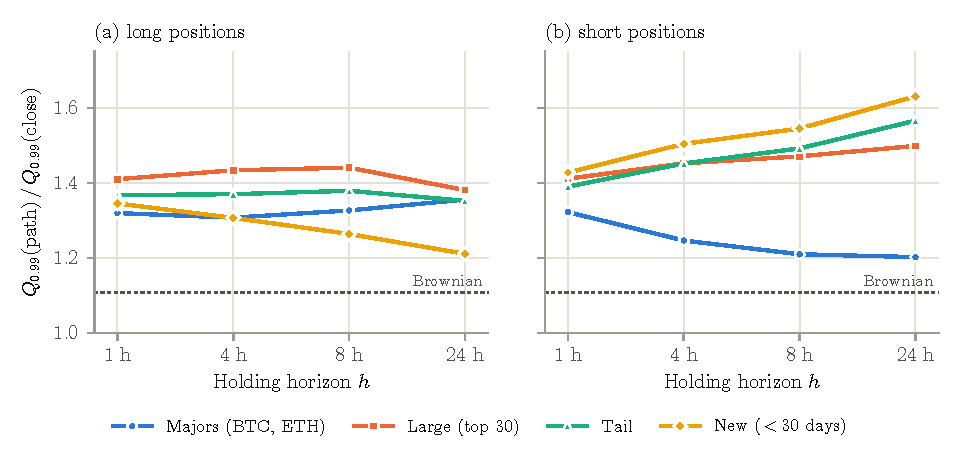
\includegraphics[width=\linewidth]{figures/fig3_quantile_multiple.pdf}
\caption{Path-to-close quantile multiple $\kappa_{0.99}$ by holding horizon. Dotted line: Brownian
benchmark, $1.107$.}
\label{fig:quantiles}
\end{figure}

\subsection{Short positions and new listings}

The two sides behave differently. For longs, $\kappa_{0.99}$ is roughly constant across horizons.
For shorts outside the Majors tier, it rises with the horizon, from about 1.4 at one hour to
1.5--1.6 at 24 hours, and is highest for new listings, at 1.63. Upward spikes that subsequently
fade, typical of squeezes in thin and newly listed contracts, liquidate short positions without
leaving a trace in the terminal price.

\section{Robustness}
\label{sec:robust}

\paragraph{Survivorship.} We repeat the analysis on a balanced cohort: the 424 contracts that were
past their 30-day burn-in on 1 November 2025 and still trading on 31 October 2026. The cohort is
biased towards survivors and should therefore \emph{understate} path risk. The results change
little (Table~\ref{tab:robust}): quantile multiples move by at most about $0.05$, and unseen shares
by at most six percentage points. The findings are not an artefact of the changing universe.

\paragraph{Mark price versus traded price.} All results use the mark price, on which liquidation is
triggered. The mark price is a smoothed construction; on Binance it is a median of index-based
estimates and the contract price~\cite{binance-mark}. Measured on last traded prices instead,
close-to-close risk is almost unchanged but path risk rises: for a 10x long held one hour, $U$
increases from 51\% to 59\% in the Large tier and from 55\% to 63\% in the Tail tier
(Figure~\ref{fig:marklast}). The smoothing removes some short-lived wicks. The mark-price figures are
therefore a conservative description of the price path a trader observes; the smoothing does not
remove the effect.

\begin{table}[t]
\centering
\caption{Robustness. \emph{Mark}: main study. \emph{Cohort}: mark price, the 424 contracts live for
the whole period (no New tier by construction). \emph{Last}: same universe, last traded prices.
``--'': no close breach.}
\label{tab:robust}
\footnotesize
\setlength{\tabcolsep}{4.5pt}
\begin{tabular}{@{}lrrrrrrrrr@{}}
\toprule
 & \multicolumn{3}{c}{$\kappa_{0.99}$, long, 1 h} & \multicolumn{3}{c}{$U$, 10x long, 1 h} & \multicolumn{3}{c}{$\kappa_{0.99}$, short, 24 h} \\
\cmidrule(lr){2-4}\cmidrule(lr){5-7}\cmidrule(lr){8-10}
Tier & Mark & Cohort & Last & Mark & Cohort & Last & Mark & Cohort & Last \\
\midrule
Majors & 1.32 & 1.32 & 1.35 & -- & -- & -- & 1.20 & 1.20 & 1.22 \\
Large & 1.41 & 1.41 & 1.51 & 51\% & 57\% & 59\% & 1.50 & 1.45 & 1.53 \\
Tail & 1.37 & 1.37 & 1.47 & 55\% & 57\% & 63\% & 1.57 & 1.60 & 1.60 \\
New & 1.35 & -- & 1.43 & 52\% & -- & 59\% & 1.63 & -- & 1.66 \\
\bottomrule
\end{tabular}

\end{table}

\begin{figure}[t]
\centering
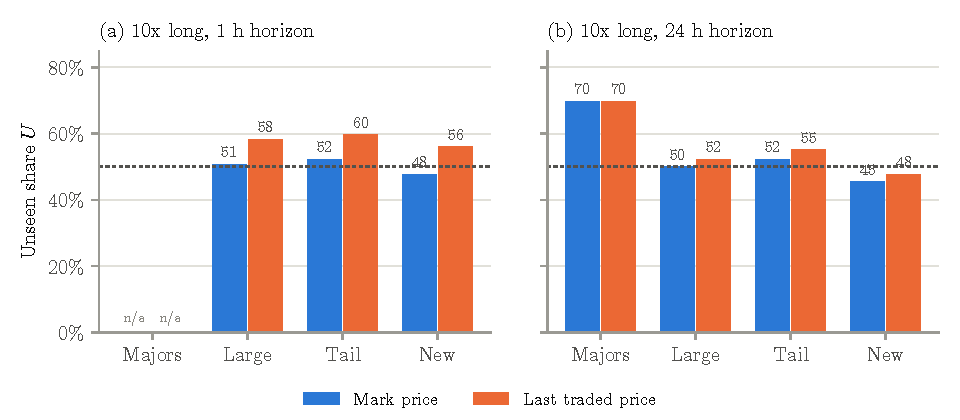
\includegraphics[width=\linewidth]{figures/fig4_mark_vs_last.pdf}
\caption{Unseen share $U$ for a 10x long, measured on the mark price and on the last traded price.
Dotted line: Brownian benchmark. Majors at one hour: no close breach.}
\label{fig:marklast}
\end{figure}

\section{Implications for risk measurement}

\begin{enumerate}\itemsep2pt
\item \textbf{Measure the path, not the close.} Value-at-risk and volatility for leveraged positions
should be estimated from the running extremum of the price over the holding period, or from
range-based estimators~\cite{parkinson,garmanklass,rogerssatchell}, not from terminal returns alone.
\item \textbf{Match the horizon to the monitoring.} Liquidation is a first-passage event under
continuous monitoring. A daily risk figure describes the end of the day; the position must survive
every instant before it.
\item \textbf{Scale terminal tails, asymmetrically.} Where only close-to-close statistics are
available, these data indicate that the 1-in-100 adverse excursion is 20--45\% larger than the
terminal loss for longs, and up to 63\% larger for shorts in thin or newly listed contracts.
\item \textbf{Treat new listings as a separate regime.} The first 30 days carry the highest
close-to-close risk and the heaviest path tail for short positions.
\end{enumerate}

\section{Limitations}

Maintenance-margin rates are representative per tier rather than each contract's tiered schedule,
and the Tail and New rates are below Binance's current median, which makes the breach probabilities
conservative. Fees, funding and liquidation penalties are ignored. Positions use isolated margin;
cross margin pools collateral and changes the boundary. The study covers one venue and one year. The
liquidity threshold (\$5 million a day) and the 30-day burn-in are design choices; the
balanced-cohort check suggests that the conclusions do not depend on the composition of the
universe.

\paragraph{Reproducibility.} All results are computed from public data by an open pipeline, from
download to the figures and tables in this paper: \url{https://github.com/PTR-25/crypto-path-risk}.

\begin{thebibliography}{99}\small\raggedright
\bibitem{binance-liq} Binance. Binance Futures liquidation protocols. Help centre,
\url{https://www.binance.com/en/support/faq/360033525271}, accessed 22 November 2026.
\bibitem{binance-mark} Binance. What are mark price and price index in USD-margined futures? Help
centre, \url{https://www.binance.com/en/support/faq/360033525071}, accessed 22 November 2026.
\bibitem{binance-brackets} Binance. Futures leverage and margin brackets, public feed of the Leverage
\& Margin page, \url{https://www.binance.com/bapi/futures/v1/friendly/future/common/brackets},
retrieved 22 November 2026.
\bibitem{bybit-mark} Bybit. Mark price calculation (perpetual contracts). Help centre,
\url{https://www.bybit.com/en/help-center/article/Mark-Price-Calculation-Perpetual-Contracts},
accessed 22 November 2026.
\bibitem{bybit-api} Bybit. V5 API, instruments info,
\url{https://api.bybit.com/v5/market/instruments-info?category=linear}, retrieved 22 November 2026.
\bibitem{okx-liq} OKX. System liquidation mechanism. Help centre,
\url{https://www.okx.com/en-us/help/system-liquidation-mechanism-eea}, accessed 22 November 2026.
\bibitem{okx-api} OKX. V5 API, public instruments,
\url{https://www.okx.com/api/v5/public/instruments?instType=SWAP}, retrieved 22 November 2026.
\bibitem{deribit-api} Deribit. API v2, public/get\_instruments,
\url{https://www.deribit.com/api/v2/public/get_instruments?currency=USDC&kind=future}, retrieved 22
November 2026.
\bibitem{hl-liq} Hyperliquid. Liquidations. Documentation,
\url{https://hyperliquid.gitbook.io/hyperliquid-docs/trading/liquidations}, accessed 22 November
2026.
\bibitem{hl-api} Hyperliquid. Info endpoint, perpetuals metadata,
\url{https://api.hyperliquid.xyz/info}, retrieved 22 November 2026.
\bibitem{bgk} M.~Broadie, P.~Glasserman and S.~Kou. A continuity correction for discrete barrier
options. \emph{Mathematical Finance} 7(4), 325--349, 1997.
\bibitem{garmanklass} M.~B.~Garman and M.~J.~Klass. On the estimation of security price
volatilities from historical data. \emph{Journal of Business} 53(1), 67--78, 1980.
\bibitem{parkinson} M.~Parkinson. The extreme value method for estimating the variance of the rate
of return. \emph{Journal of Business} 53(1), 61--65, 1980.
\bibitem{rogerssatchell} L.~C.~G.~Rogers and S.~E.~Satchell. Estimating variance from high, low and
closing prices. \emph{Annals of Applied Probability} 1(4), 504--512, 1991.
\end{thebibliography}

\appendix
\section{Liquidation boundaries}

\begin{table}[H]
\centering
\caption{Adverse move to liquidation $d_\ell$ for a long position, in \%, by tier maintenance-margin
rate $m$ and leverage. ``--'': not admissible ($1/L\le m$). Short-side boundaries are
$d_s=d_\ell(1-m)/(1+m)$.}
\label{tab:liq}
\footnotesize
\begin{tabular}{@{}rrrrrrrrrr@{}}
\toprule
$m$ & Contracts & Max lev. & 10x & 20x & 25x & 50x & 75x & 100x & 150x \\
\midrule
0.40\% & 2 & 150x & 9.64 & 4.62 & 3.61 & 1.61 & 0.94 & 0.60 & 0.27 \\
0.50\% & 18 & 100x & 9.55 & 4.52 & 3.52 & 1.51 & 0.84 & 0.50 & 0.17 \\
0.60\% & 10 & 75x & 9.46 & 4.43 & 3.42 & 1.41 & 0.74 & 0.40 & 0.07 \\
0.65\% & 8 & 75x & 9.41 & 4.38 & 3.37 & 1.36 & 0.69 & 0.35 & 0.02 \\
1.00\% & 136 & 75x & 9.09 & 4.04 & 3.03 & 1.01 & 0.34 & -- & -- \\
1.20\% & 2 & 35x & 8.91 & 3.85 & 2.83 & 0.81 & 0.13 & -- & -- \\
1.50\% & 193 & 50x & 8.63 & 3.55 & 2.54 & 0.51 & -- & -- & -- \\
2.00\% & 131 & 25x & 8.16 & 3.06 & 2.04 & -- & -- & -- & -- \\
2.50\% & 229 & 20x & 7.69 & 2.56 & 1.54 & -- & -- & -- & -- \\
3.00\% & 12 & 20x & 7.22 & 2.06 & 1.03 & -- & -- & -- & -- \\
4.00\% & 7 & 20x & 6.25 & 1.04 & -- & -- & -- & -- & -- \\
5.00\% & 160 & 10x & 5.26 & -- & -- & -- & -- & -- & -- \\
8.00\% & 2 & 8x & 2.17 & -- & -- & -- & -- & -- & -- \\
10.00\% & 17 & 5x & -- & -- & -- & -- & -- & -- & -- \\
\bottomrule
\end{tabular}

\end{table}

\end{document}
